\documentclass[11pt,a4paper,titlepage]{article}
\renewcommand{\familydefault}{\sfdefault}
\usepackage[margin=0.75in]{geometry}
\usepackage{courier}
\usepackage[english]{babel}
\usepackage[utf8]{inputenc}
\usepackage{fancyhdr}
\usepackage{graphicx}
\usepackage{listings}
\usepackage{color}
\usepackage{hyperref}

\hypersetup{
    colorlinks=true,
    linkcolor=blue,
    filecolor=magenta,      
    urlcolor=cyan,
}
 
\urlstyle{same}

\setlength{\headheight}{16pt}

\definecolor{codegreen}{rgb}{0,0.6,0}
\definecolor{codegray}{rgb}{0.5,0.5,0.5}
\definecolor{codepurple}{rgb}{0.58,0,0.82}
\definecolor{backcolour}{rgb}{0.95,0.95,0.92}

\lstdefinestyle{mystyle}{
    backgroundcolor=\color{backcolour},
    commentstyle=\color{codegreen},
    keywordstyle=\color{magenta},
    numberstyle=\tiny\color{codegray},
    stringstyle=\color{codepurple},
    basicstyle=\footnotesize\ttfamily,
    breakatwhitespace=false,
    breaklines=true,
    captionpos=b,
    keepspaces=true,
    numbers=left,
    numbersep=5pt,
    showspaces=false,
    showstringspaces=false,
    showtabs=false,
    tabsize=2
}
\lstset{style=mystyle}

\pagestyle{fancy}
\fancyhf{}
\rhead{Energy Web Foundation}
\lhead{EWF Authority Nodes}
\rfoot{Page \thepage}

\begin{document}
\title{EWF Authority Nodes - Requirements and Procedures}
\author{Markus Keil, Friedrich Raschwitz}
\date{January 2019}

\maketitle

\begin{abstract}
To provide a stable and secure blockchain for all affiliates and customers, it is important that all parties that run authority nodes follow the procedures and guidelines written in this document.
Authority nodes are not used for interaction with the chain. If an affiliate wants to access the chain via RPC through a central node it has to be set up separately as non-authority.
\end{abstract}

\tableofcontents

\newpage
\section{Nomenclature}

\begin{description}
    \item[EWF Network Operations (NetOps)] 
        Group of people on EWF side with the responsibility to keep the blockchain secure and operational at all times.
    \item[EWF Governance Operations (GovOps)] 
        Group of people on EWF side that decide on governance questions.
    \item[NodeControl] 
        A system component that carries out operational tasks on a validator node on behalf of NetOps
    \item[Bootnode] 
        Parity node that runs in fullnode configuration and is part of the bootnode section of the chainspec file.
        New clients that join the chain will contact a bootnode to discover other nodes on the network that are known to the bootnode.
    \item[Validator Node]
        Parity node that seals transactions into new blocks based on the AURA consensus algorithm.
    \item[Genesis Node]
        A special validator node. The genesis nodes are the first ones on the network and operated by EWF. These nodes will bootstrap the blockchain with the genesis block.
    \item[Fullnode]
        A simple node on the network that don't seal new blocks. These nodes are not in the scope of these guidelines
    \item[Supportnode]
        A host that runs auxiliary services like IPFS or Incubed Server

\end{description}

\newpage
\section{System Design}

The system of the validator nodes and their supporting components are designed to provide security and stability. The basic layout is shown in Figure ~\ref{fig:sysdesign}.
Also along the active validator set is a set of standby validator nodes called Shadow Validators, that can swap in for any failed or otherwise compromised validator.

\begin{figure}[ht]
	\centering
    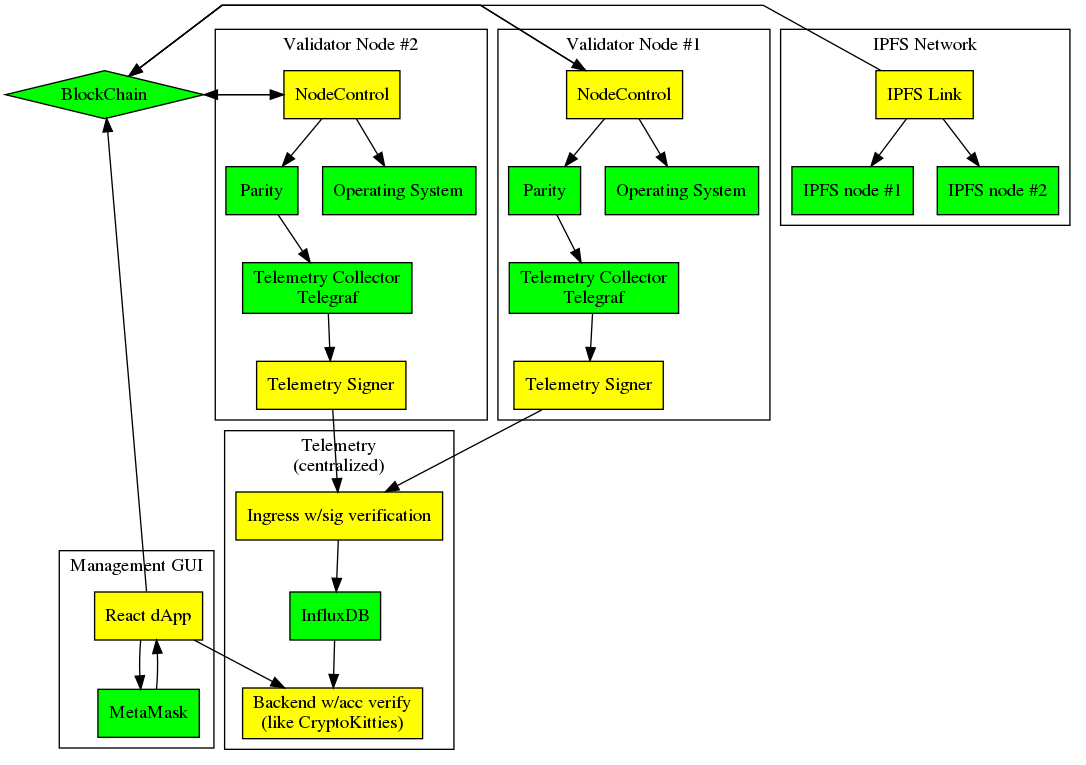
\includegraphics[width=0.85\textwidth,keepaspectratio]{./images/sys-diagram.png}
	\caption{Validator System Design}
	\label{fig:sysdesign}
\end{figure}

\subsection{Shadow Validators [Not part of MVP]}

As running hundreds of validators at the same time increases network traffic and also time to finality a lot, the concept of shadow validators can be used to have a small set of 23 active validators and a number of dormant shadow validators.

During onboarding an affiliate can choose either to run a single validator node or provide resources for two validator nodes from which only one gets enlisted into the active validator set.
The second node is also completely onboarded but would run with the sealer disabled. 
It would be just a normal peer acting as a full node (as any other validator would).
If another validator node would go offline or start misbehaving, the network starts to counteract this behavior by activating a shadow validator, while in the same time remove the misbehaving validator from the active set. This will happen automatically via the validator smart contract. To ensure the network can heal it self this way, the validator address of the shadow node is recorded to the validator contracts shadow node list, from which it then can draw new nodes. The contract will emit a wake up event that will be picked up by NodeControl on the dormant validator node and restarts the blockchain client with the sealer enabled. NodeControl reports back successful activation to the validator contract which then will add the now active shadow node to the active list of validators. Along with the wakeup event a disable event is recorded on chain for the misbehaving one.

The main purpose of this is to counteract single-node attacks, where one node is brought down due to some kind of DoS attack. 
Once the attacked node is back up again and re-validated by NetOps, it can replace the activated shadow node  which then would go back to be dormant. \\

Additional idea is to use this mechanism to swap random nodes in and out of the shadow set on a regular basis. Governance has to make sure that over the period of a year each validator had an equal share of "active time" to evenly distribute transaction fees and block rewards.


\subsection{System Components}
\label{components}

These system components are tailor made or where developed for the validator network.

\subsubsection{NodeControl}

A small deamon that will carry out updates on behalf of NetOps. See \ref{nodecontrol}.

\subsubsection{Telemetry Signer}

System telemetry is collected using Telegraf. But to ship the telemetry, Telegraf won't send it directly to the telemetry backend but instead to a local deamon called "Telemetry Signer".
This deamon will make sure that telemetry is only send to a verified telemetry collection endpoint (Telemetry Ingress) using TLS certificate fingerprints.
Each telemetry package send to the Ingress will be signed by the telemetry signer.

\subsubsection{Telemetry Ingress}

A deamon that will wait for connections from telemetry signers. It will verify the signature of each incoming telemetry package before inserting it into the InfluxDB telemetry datastore. If the signature is not valid it will report this to a log file.

\subsubsection{IPFS Link [Not part of MVP]}

IPFS Link is a service that allows human readable urls to be resolved to IPFS hashes. It is used in this system to provide the link to the NetOps Management dApp. This way the management dApp can be hosted decentralized to increas reliability.

\subsection{Other Components}

These components are standardize open-source components.

\subsubsection{IPFS [Not part of MVP]}

IPFS is used to distribute the management ui. A central support node would provide an IPFS node that is connected to the public IPFS network. The management UI would be accessed either through a local IPFS client or trough a public IPFS gateway.
This way the UI stays accessible, even when the support node fails.

\subsubsection{Telemetry Collector}

The system uses Telegraf to collect the telemetry from on the nodes. This collected data is then send via the InfluxDB wire protocol to the also locally running telemetry signer.

\subsubsection{Grafana [Only MVP]}

To visualize the telemetry the telemetry node will run a Grafana instance. In a later milestone this then could be replaced or integrated into the governance dApp.

\subsubsection{Blockchain Client}

The blockchain client is the main component of the system as it provides the connection to the blockchain and also carries out signing and validation duties. 
The probably used software will be Parity-Ethereum from Parity Tech running the AURA Proof-of-Authority engine.


\newpage
\section{NodeControl}
\label{nodecontrol}

NodeControl is a small management application that runs on each validator node. It is in charge of carrying out simple update tasks.
It will listen to the local blockchain client via the HTTP RPC interface. If the local blockchain is not available it will fallback to the Incubed network to receive and verify update events \footnote{Incubed and this feature are not part of the MVP}.
The ethereum address of the validator account is used as a node identifier. NodeControl will only act on events directly directed to its assigned address.
This allows granular deployment of updates. \\

NodeControl will also track the local blockchain client to determine the current number of validators \footnote{MVP will have a fixed, configurable number of block to determine finality}. This is needed to determine finality of an update command.
The trigger process is shown in Fig. ~\ref{fig:nctrigger}.


\begin{figure}[ht]
	\centering
    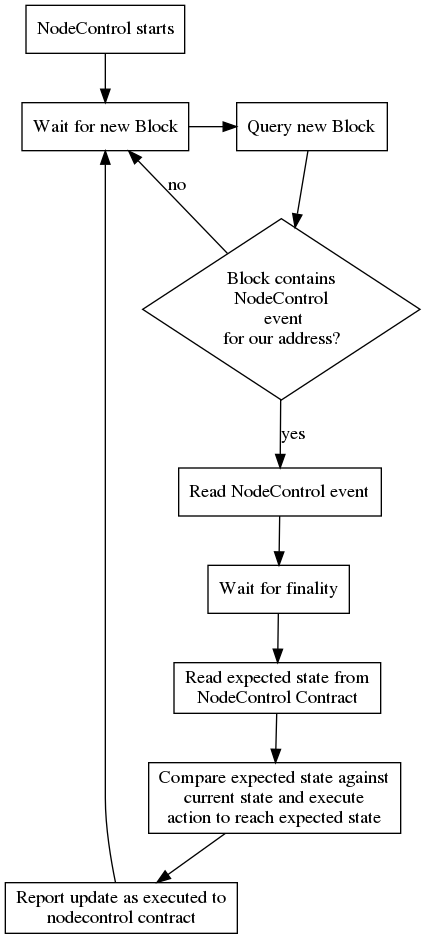
\includegraphics[height=0.65\textheight,keepaspectratio]{./images/nodecontrol.png}
	\caption{NodeControl Trigger Process}
	\label{fig:nctrigger}
\end{figure}

\newpage
\subsection{Interface to Contract}

This is an abstract definition of the Smartcontract interface between the NodeControl deamon and the accompanying contract on-chain.

\begin{itemize}

    \item \texttt{event UpdateAvailable(address targetValidator, unit eventId)} \\
    The contract has to emit this event once an update should be triggered on a node. If one would like to update multiple validators at once the event has to be send for each node individual.

    \item \texttt{function RetrieveUpdate(address targetValidator, unit eventId)} \\ \texttt{returns (uint command, byte[] payloadHash, string payload)} \\  
    NodeControl will call this function after finality has been reached to retrieve the actual command and payload. \\
    Command is an \texttt{uint} based on this map: \\
    \texttt{0 => updateParity} Will update the parity docker container. \\
    \texttt{1 => updateChainspec} Will update the chainspec file. \\
    \texttt{2 => enableSigner} Will restart Parity with signing enabled (payload and hash empty) \\
    \texttt{3 => disableSigner} Will restart Parity with signing disabled (payload and hash empty) \\

    The command code will also determine the meaning of the two remaining fields \texttt{payloadHash} and \texttt{payload}.

    \begin{itemize}
        \item \texttt{updateParity} \\
        \texttt{payloadHash} => The SHA256 Id of the docker image returned by \texttt{docker image inspect} \\
        \texttt{payload} => The dockerimage from dockerhub including tag (eg. \texttt{parity/parity:v2.2.5})

        \item \texttt{updateChainspec} \\
        \texttt{payloadHash} => The SHA256 hash of the downloaded file \\
        \texttt{payload} => HTTPS url to download the new chainspec 

    \end{itemize}
    
    \item \texttt{function ConfirmUpdate(unit eventId, boolean success)} \\
    After NodeControl carried out the update it will report back with a transaction calling this function. It will send a boolean if the update was successful or not. The transaction will be send from the validator account over HTTP RPC.

\end{itemize}

\newpage
\section{Genesis Network}

The Genesis Network is a special set of validators and full nodes that will be used during launch. Hosts of the genesis network will be geographically distributed across different AWS regions. These regions will be linked via VPC peering, so traffic inside the genesis network is not public facing. \\

The genesis network will be run by the EnergyWeb Foundation.

\begin{figure}[ht]
	\centering
    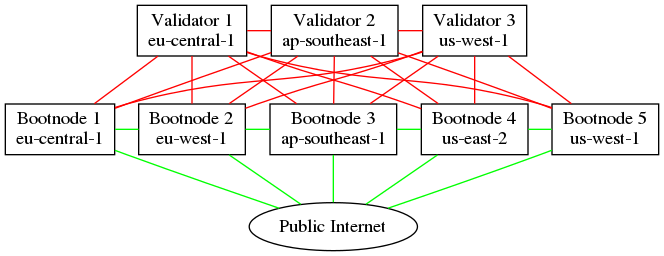
\includegraphics[width=0.85\textwidth,keepaspectratio]{./images/genesis-network.png}
	\caption{Genesis Network Layout}
	\label{fig:genesisnet}
\end{figure}

\subsection{Validators}

The genesis validators will be starting the chain and also their validator account addresses are hard coded as constructor arguments to the validator contract in the chain specification. The hosts running those validator nodes adhere to the same security standards as normal validators with the addition that they don't have any connection to the public internet blockchain wise. \\
The following outgoing traffic is permitted though an AWS NAT gateway:

\begin{itemize}
    \item DNS (63/UDP)
    \item HTTPS (443/TCP) - mainly for sys updates
\end{itemize}

Blockchain traffic is only allowed inside the AWS VPC to the Bootnodes. The validators will have a special configuration file for parity to facilitate that along with the following security group settings

\begin{itemize}
    \item Allow P2P traffic (30303/tcp+udp) inbound only from the bootnodes via RFC1918 inside the VPC
    \item Allow P2P traffic (30303/tcp+udp) outbound only to the bootnodes via RFC1918 inside the VPC
    \item Allow SSH traffic only inbound via a jump host inside the VPC over RFC1918
\end{itemize}

A preferred EC2 Instance type would be i3.xlarge (4 cores - Xeon E5 2686v4, 30GB RAM, 950GB NVMe SSD). These nodes also don't have dedicated public IP's

\subsection{Bootnodes}

The genesis bootnodes are regular fullnodes (state pruned, no tracing, no fatdb, no warp).
They accept connections from the public internet and the validator VPC's on their blockchain P2P port.

Enode addresses of those bootnodes will be part of the general public chainspec.


\newpage
\section{Threat model}

This section describes potential attack vectors to the system and how they are either mitigated by the system design, automatic intervention or human intervention.

\subsection{Telemetry}

As telemetry needs to flow from the validators to a single ingress point on the management system it is not protected by decentralization.
This telemetry helps to detect abnormalities in the operation of the validators caused by either system malfunction or deliberate attacks.

\begin{description}
    \item[Sending tampered data] 
        If an attacker manages to disturb node operation, he might try to disguise this by sending normal looking telemetry to the telemetry ingress on behalf of the attacked node. NetOps would detect the faulty node with increased time delay as telemetry data would contradict actual node behavior. \\
        \textbf{Prevention:} Each telemetry package will be signed with the validators private key and verified by telemetry ingress. This way an attacker is not able to send tampered telemetry on behalf of a node.
    
    \item[Denial-of-Service against the telemetry ingress] 
        An attacker might try to bring down the telemetry ingress completely to "blind" the EWF NetOps team about the status of the validator network. \\
        \textbf{Mitigation:} Telemetry senders on the validators will keep track of connection failures to the telemetry ingress. If the connection is unstable or down for a particular amount of time the node will send periodically (<10 minutes) basic health metrics via a second channel (eg. E-Mail).
        EWF NetOps has access to this channel and can at least verify basic health of the system.

    \item[Phishing for telemetry] 
        An attacker might try to receive telemetry from a node by re-routing telemetry traffic to an attacker system that mimics the ingress (DNS spoofing, MITM). The attacker can gain knowledge about for example the systems load patterns or how a system might respond to an attack. \\
        \textbf{Prevention:} Connection between telemetry sender and telemetry ingress is HTTPS. The SHA256 fingerprint of the ingress certificate is verified against the known good fingerprints.
        The fingerprint gets deployed along with the telemetry sender component and can only be updated through an update request from the blockchain.
        
    \item[DNS-Spoof/MitM against GUI] 
        An attacker might manage to DNS Spoof/MitM the connection between the browser of a member from the NetOps team and the telemetry backend. This way the attacker could present a faked system state of the validator network to NetOps. \\
        \textbf{Prevention:} Each JSON response from the telemetry backend needs to carry a signature for the payload that can be verified by the management dApp

    \item[Unauthorized access to telemetry data]
        Telemetry data should only be available to the EWF NetOps Team. An attacker might try to directly call the telemetry backend to receive the data. \\
        \textbf{Prevention:} The telemetry backend will present a challenge to the GUI which the EWF NetOps team member has to sign with his private key using metamask. This challenge+signature is then send along with all following requests and verified against a smart contract.

\end{description}

\subsection{Node Control}

The Node control component is used to carry out updates to the validator nodes. These updates need to be legitimized by the EWF NetOps and GovOps teams.
The component has the potential to disable a node due to a faulty or malicious update .

\begin{description}
    \item[Send fake update event] 
        An attacker might try to fool the NodeControl into carrying out an update script that is not approved. \\
        \textbf{Prevention:} NodeControl will talk to its local blockchain client most of the time via IPC. 
        If it has to talk to outside nodes because the local client is down, it'll use incubed to verify responses.

    \item[Compromised Payload]
        An attacker might MitM traffic to any server NodeControl would download a payload from (mainly used for the chain spec file update process). \\
        \textbf{Containment:} Each update will have the SHA256 hash of its agreed payload on chain. The payload downloaded by NodeControl is verified against this hash. If the hashes don't match NodeControl will not carry out the command and report a faulty update to the NodeControl Contract.

\end{description}


\subsection{Management GUI/dApp}

The Management GUI is the central hub for the NetOps team to verify healthiness and current operational status of the validator network. Therefore it has a high requirement on reliability.

\begin{description}

    \item[Server delivering UI to NetOps is not available] 
        An attacker might be able to DDoS the Server/CDN or otherwise disturb connection to the assets needed to run the management dApp. \\
        \textbf{Prevention:} The dApp itself is hosted on IPFS. Therefore taking down a single UI serving node won't disturb operation. For improved reliability NetOps members should run their own local IPFS nodes and use the IPFS companion extension,
        This allows the local IPFS node to be used to deliver the GUI to the browser. 

    \item[Deliver malicious dApp to NetOps team] 
        An attacker might be able to deliver a malicious dApp to the NetOps team. With this it might be possible to deceive NetOps about the current status of the validator network or have them sign bogus update commands.  \\
        \textbf{Prevention:} Provide a local bootstrap copy of the index.html page that loads the dApp from IPFS, preferably with a local IPFS node. Have hardcoded checksums of those files in the index.html and verify payload during load as the attacker could intercept HTTPS traffic to the IPFS gateways or the local node and deliver a malicious asset to the browser.

\end{description}


\subsection{Other Attack Vectors}

This section consolidates attack vectors that are either not specific to a single component or targeted against miscellaneous components.


\begin{description}

    \item[Attack time servers] 
        The Aura PoA consensus algorithm highly depends on accurate system clocks. An attacker could try to manipulate the system clock by intercepting requests made by the operating system via NTP (Network Time Protocol). If the attacker shifts the system time by +block time or -block time the validator will start signing during the wrong slot. Other validators then won't accept that block because it is out-of-turn and vice-versa the manipulated node would mark all incoming blocks as invalid as from its point of view all other validators appear to be syncing out-of-turn. \\
        \textbf{Mitigation:} Some validator nodes should use high-precision hardware clocks such as GPS-based ones or DCF-77 clocks instead of NTP for their time source. This way not the whole network is affected. Normal operation could be restored by removing all non-precision-clock nodes from the network. This could mean reduced chain performance.

\end{description}


\newpage
\section{Incentivation}

The EWF chain knows four levels on nodes:

\begin{itemize}
    \item The double-validator with an active sealer and a shadow node
    \item The single validator with only the active sealer
    \item A support node running a non-sealing full node along with an IPFS and InCubed server. Support nodes don't need to fulfill the higher security standards that validator nodes need to provide.
    \item plain non-validator nodes, which are just normal blockchain client nodes that don't need to adhere to any increased security standards. They can be run by anybody and therefore are not part of these guidelines.
\end{itemize}

Best case scenario would be that every affiliate runs the double validator configuration along with a separate support node. This would take 3 separate hosts the affiliate has to maintain.
Each affiliate should at least run a support node as it the easiest configuration to run and to secure.

The target for the active validator set should be at 25 validator nodes with the same amount of shadow nodes.


\newpage

\section{Validators run by Affiliates}

This section will go through the requirements needed to run a standard validator by an EWF affiliate.

\subsection{Hardware/VM selection for Validators}

Affiliate can choose to run the node either On-Premise on their own hardware or at one of the supported cloud-providers.

\subsubsection{On-Premise}

A on-premise node should have these specs or higher. These resources should be reserved for the validator node and not shared with other workloads.

\begin{enumerate}
    \item Modern Multi-core x64 CPU (at least 4 threads, preferably Xeon-class)
    \item 8GB RAM (preferably ECC)
    \item Local SSD storage, 250GB free capacity for blockchain, redundant in RAID-1
    \item 1 GBit NIC
\end{enumerate}

\subsubsection{Amazon AWS}

The following EC2 instance sizes are appropriate to run validators:

\begin{itemize}
    \item m5.xlarge
    \item m5.2xlarge
    \item m5a.xlarge
    \item m5a.2xlarge
    \item c5.xlarge
    \item c5.2xlarge
\end{itemize}

The default EBS storage assigned (normally 8GB) is not large enough to run the node. Make sure to run the node with following EBS storage settings:
\begin{itemize}
    \item General Purpose SSD (gp2)
    \item at least 300GB size
\end{itemize}

\subsubsection{Microsoft Azure}

The following Azure VirtualMachine sizes are suitable to run a validator:

\begin{itemize}
    \item D4s\_v3
    \item DS3\_v2
    \item B4ms
\end{itemize}

Use \textbf{Premium SSD} as attached storage with a size of at least \textbf{300GB}.

\subsection{Reliability and Diversity}

EWF NetOps will guarantee a certain reliability and diversity by enforcing heterogeneity of geographical location, Operative System and cloud service. The rationale is that a bug of a specific OS, a failure of a cloud service provider or the backbone internet service provider should not harm the consensus of the Validators. \\
For this reason, NetOps establishes a set of rules:

\begin {itemize}
    \item There are at least two Validators running different OS in the system.
    \item The second most common OS is run by at least 20\% of Validators.
    \item There are at least 15\% Validators operating from America, 15\% from Europe and 15\% from Asia.
    \item At least two cloud services are used. The second most popular is used by at least 20\% of the Validators.
\end{itemize}
\subsection{Supported Operating Systems}

The following Linux-based Operating Systems are supported for running a authority node: 

\begin{itemize}
    \item Ubuntu Server 18.04 LTS
    \item Debian 9.8
    \item CentOS 7
\end{itemize}

Affiliates can apply for a certain operating system, but in order to keep a heterogeneous infrastructure EWF NetOps can instruct the Affiliate to use a specific operating system from the above list. 
The operating system must be installed according to the settings described in this document to qualify the host for becoming part of the authority network.


\subsection{Security Requirements}

Running an authority nodes requires raised awareness of host and node security as authorities are a main attack surface to disturb operation of the block chain.
The following security rules apply:

\begin{itemize}
    \item No services are permitted to run on the same host that are not part of the authority node package
    \item All incoming connections on all ports except SSH (22/tcp) and the P2P (30303/tcp+udp) port have to be firewalled on the host with DROP rules. To guarantee proper network etiquette, incoming ICMP has to be accepted.
    \item SSH access is only allowed for non-root users
    \item SSH access is only allowed through RSA keys
    \item Parity RPC endpoints (HTTP, WebSocket) have to be disabled
    \item System updates have to applied regularly and in a timely manner
    \item Regular run of rootkit detectors
\end{itemize}

Most of these rules will be provided in the following set up guides.
\subsection{Connectivity Requirements}

The following requirements should be met to ensure proper operation:

\begin{itemize}
    \item Wired connection with 100 MBit/s symmetric link to the internet
    \item Low latency connection to next internet hop (<5ms)
    \item No data volume limitations
\end{itemize}

Even this document requires a 100MBit/s connection, that connection will not be saturated by the node. You can expect ~10-30MBit/s \footnote{TODO: need to verify} when the chain is under load. 
Traffic will mainly flow on port 30303 (udp/tcp). If chosen to run on a cloud provider, EWF NetOps needs to be consulted to select an appropriate hosting region to ensure node distribution across multiple regions.
If chosen to run on-premise, EWF NetOps has to be informed about the hosting location to ensure proper global distribution decisions can be made.
The hosting location should be chosen to be as close as possible to one of the major internet exchanges:

\begin{itemize}
    \item Germany/Continental Europe/USA - DE-CIX / AMS-IX
    \item United Kingdom - LINX
\end{itemize}
\subsection{AWS Security}
When using EC2 instances one can provide at least one additional layer of security using a virtual firewall. The access of administrative tasks outside of the virtual OS also needs to be taken care of.

\subsubsection{Access Management Recommendations}
\begin{enumerate}
    \item Do not use the root account for managing EC2 instances, instead assign a new user administrative rights for doing that.
    \item Use groups to manage permissions with multiple users and always keep the set of permissions to a minimum
    \item Enable multi-factor authentication for administrative accounts
    \item Regularly check logs regarding account activity, e.g. using Cloudfront \href{https://docs.aws.amazon.com/AmazonCloudFront/latest/DeveloperGuide/AccessLogs.html}{AWS Docs: Access Logs}
\end{enumerate}

\subsubsection{AWS Firewall}

AWS provides an alternative firewall solution for their virtual OS. Instead of configuring the firewall in the OS itself (or additionally), one can configure it one layer above. This firewall is defined by a set of "security groups". Each security group contains rules what packets should be permitted to or from the EC2 instance. That means that instead of having a set of 'Allow' or 'Deny' rules security groups can only contain 'Allow' rules while everything else is denied by default. \\

That also means that by default SSH access needs to be allowed in one security group. More information on that can be found here: \\ 
\href{https://docs.aws.amazon.com/AWSEC2/latest/UserGuide/authorizing-access-to-an-instance.html}{AWS Docs: authorizing-access-to-an-instance}

\subsubsection{EC2 Key Pairs}
EC2 key pairs are basically just RSA key pairs generated and distributed using AWS-specific commands. In general one can follow the guide in the SSH section. However, these commands may be more convenient to some users, more information here: \\
\href{https://docs.aws.amazon.com/AWSEC2/latest/UserGuide/ec2-key-pairs.html}{AWS Docs: ec2-key-pairs}



%\newpage
%\newcommand{\code}[1]{\texttt{#1}}
\section{SSH Setup}
A safe access is needed when interacting with remove machines. SSH is one of the most widely used programs for this purpose. It is found in the software repositories of most Linux-based OS. \\
By default SSH uses password-based access, however in this section a better approach based on RSA key-pairs is shown.

\subsection{Clientsetup}
The client has to prove to the server that he is in the possession of a private key which corresponds to a public key on the server.
\begin{enumerate}
    \item{\textbf{Installation}}\\
        The package openssh-client is needed.\\
Debian or Ubuntu: \\
\code{
    \# apt-get install openssh-client \\
}
Fedora: \\
\code{
    \# yum -y install openssh-client \\
}
Create the .ssh folder in the home directory if not present. \\
    \item{\textbf{Generating the keypair}}\\
Then to create a RSA keypair do: \\
\code {
    \# ssh-keygen -t rsa -b 4096 -f ~/.ssh/\textit{filename} \\
}
This will generate a 4096 bit sized RSA key-pair with a filename of your choosing, after asking for a passphrase. By default the command would generate a private key with the filename "id\_rsa" and insert it into .ssh, but in case of using several RSA keys it is better to differentiate between them.  \\
The private key has to have permissions set to 600:\\
\code{
    \# chmod 600 \textit{filename}
}
    \item{\textbf{Configuration}}\\
To tell SSH which key should be used a config file needs be created. It also allows creating an SSH connection using a shorter name for the host instead of writing the full domain or IP.\\
Add a file in .ssh with the name "ssh\_config" with the following content:\\
\code{
    Host \textit{servername}
}\\ \indent
 \hspace{15pt}\code{
    HostName \textit{server-domain}
} \\ \indent
\hspace{15pt}\code{
    User \textit{remote-username}
} \\ \indent
\hspace{15pt}\code{
    Identityfile \textit{~/.ssh/filename}
} \\
The "Host" option can be any name of your choosing, e.g. "ewf-node". "Hostname" is the address of the server and "User" is the username on that server. Finally, the "Identityfile" option should point to your private key. Once the server is set up a connection can be established using \code{ssh \textit{hostname}}.  \\
More information on the configuration file can be found here: \\ https://www.ssh.com/ssh/config/
\end{enumerate}
\subsection{Serversetup}
On the serverside one needs to open the SSH port and transfer the public key of the user.  \\
\begin{enumerate}
    \item{\textbf{Installation}}\\
First the server package needs to be installed: \\
Debian or Ubuntu: \\
\code{
    \# apt-get install openssh-server \\
}
Fedora: \\
\code{
    \# yum -y install openssh-server \\
}
    \item{\textbf{Configuration \& Ports}}\\
Edit the file /etc/ssh/sshd\_config and add a new line with the following option: \\
\code{
PermitRootLogin no\\
}
Then some ports need to be opened:\\
\code{
    \# iptables -A INPUT -p tcp --dport 22 -m conntrack --ctstate NEW,ESTABLISHED -j ACCEPT\\
    \# iptables -A OUTPUT -p tcp --sport 22 -m conntrack --ctstate ESTABLISHED -j ACCEPT\\
}
Save the iptables config using:
\code{
    \# service iptables save
}
\\
Next a persistent SSH service needs to be enabled: \\
\code{
    \# service ssh enable
}
    \item{\textbf{Transferring the public key}}\\
When generating a keypair using ssh-keygen, the public key is called the same as the private key, except that it has the suffix ".pub". \\
This public key needs to be transferred from the client from the client to the directory "known\_hosts" in the .ssh directory. It can be done with various means. SSH provides an dedicated command for that:\\
\code{
    \# ssh-copy-id -i \textit{path/to/public/key*} "\textit{remote-username}@\textit{server-domain}"
}
\end{enumerate}

\newpage

\subsection{Setup Procedure}

To setup a new authority node read this whole document and then use this procedure to carry out the set up. The full process is shown in Figure ~\ref{fig:onboardflow}

\begin{enumerate}
    \item Choose hosting provider (on-premise or qualified cloud provider) and favored operating system
    \item Consult with EWF NetOps on location and operating system
    \item EWF NetOps will provide the location and OS to use, along with the official installation script for the chosen operating system
    \item Install operating system according to this document
    \item Deploy blockchain node in none-validator mode using the script given by NetOps 
    \item Contact EWF NetOps to confirm installation and incoming telemetry
    \item Create Validator Keys and prepare your node configuration to switch to authority mode using the script.
    \item Send the validator account information to the EWF Governance team
    \item Re-start your node in authority-mode
\end{enumerate}

\begin{figure}[ht]
	\centering
    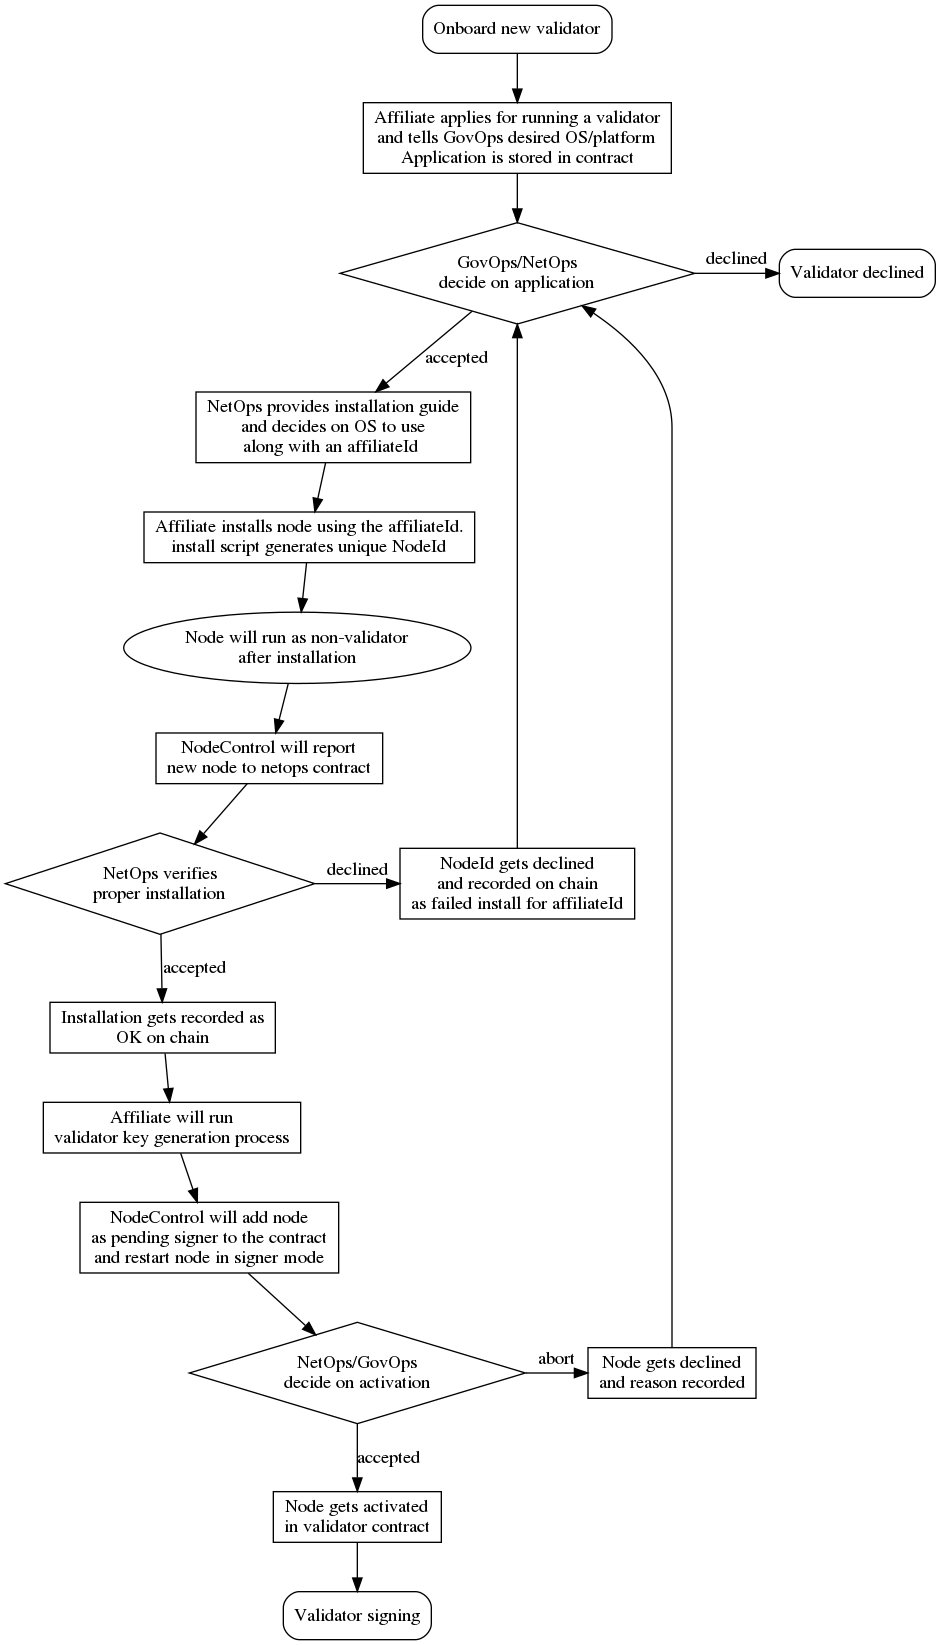
\includegraphics[width=\textwidth,height=\textheight,keepaspectratio]{./images/flow-onboard-validator.png}
	\caption{Validator On-Boarding Flow}
	\label{fig:onboardflow}
\end{figure}



\newpage
\section{Operating system installation}

The following section provide a comprehensive guide for installation of one the supported operating systems.
All further deployment procedures are based on the installation results.

\subsection{Ubuntu Server 18.04 LTS}

\subsubsection{On-Premise}

Procedure based on version 18.04.2.

\begin{itemize}
    \item Download the ISO from https://www.ubuntu.com/download/server.
    \item Boot the ISO
    \item Select \textbf{English} as language
    \item Choose a convenient keyboard layout
    \item Choose \textbf{Install Ubuntu}
    \item Let the network auto-configure -or- configure manually if needed. The system needs an internet connection.
    \item Select no proxy and keep the mirror address.
    \item Select \textbf{Use an entire disk} and confirm
    \item Choose user name and host name in next screen. Choose a strong password.
    \item Select \textbf{Install OpenSSH Server} but don't import keys   
    \item Don't select any snaps and continue
    \item Finish installation and let it boot to the prompt
    \item Login as the created user and run a full system update using \texttt{sudo apt update \&\& sudo apt dist-upgrade -y}
\end{itemize}

\subsubsection{AWS}

The Ubuntu AMI Id's for all regions in AWS can be found in Table \ref{ubuntuami}

Also Ubuntu AMI's are listed at https://cloud-images.ubuntu.com/locator/ec2/. Search for \textbf{ebs 18.04 amd64} to get the correct version.

\begin{table}[]
\centering
\begin{tabular}{ll}
Region         & AMI ID                \\
ap-northeast-1 & ami-0eb48a19a8d81e20b \\
ap-south-1     & ami-007d5db58754fa284 \\
ap-southeast-1 & ami-0dad20bd1b9c8c004 \\
ca-central-1   & ami-01b60a3259250381b \\
eu-central-1   & ami-090f10efc254eaf55 \\
eu-north-1     & ami-5e9c1520          \\
eu-west-1      & ami-08d658f84a6d84a80 \\
sa-east-1      & ami-09f4cd7c0b533b081 \\
us-east-1      & ami-0a313d6098716f372 \\
us-west-1      & ami-06397100adf427136 \\
cn-northwest-1 & ami-09b1225e9a1d84e4c \\
cn-north-1     & ami-09dd6088c3e46151c \\
us-gov-west-1  & ami-66bdd307          \\
us-gov-east-1  & ami-7bd2340a          \\
ap-northeast-2 & ami-078e96948945fc2c9 \\
ap-southeast-2 & ami-0b76c3b150c6b1423 \\
eu-west-2      & ami-07dc734dc14746eab \\
us-east-2      & ami-0c55b159cbfafe1f0 \\
us-west-2      & ami-005bdb005fb00e791 \\
ap-northeast-3 & ami-0babd61cf592f1c03 \\
eu-west-3      & ami-03bca18cb3dc173c9
\end{tabular}
\caption{Ubuntu 18.04 LTS AWS AMI Id's}
\label{ubuntuami}
\end{table}

\subsubsection{Azure}

The URN for the image is \texttt{Canonical:UbuntuServer:18.04-LTS:latest}

\subsection{Debian 9.8}

\subsubsection{On-Premise}

\begin{itemize}
    \item Download the NetInst ISO from https://www.debian.org/distrib/netinst
    \item Boot the ISO
    \item Select \textbf{Install} from the boot screen
    \item Select \textbf{English} as language
    \item Select Location based on actual location of the host
    \item Chose a convenient keyboard layout
    \item Let the network auto-configure -or- configure manually if needed. The system needs an internet connection.
    \item Name your host. Change it from \textit{debian} to something else
    \item Choose a strong root password
    \item create the user account and choose a strong password
    \item select the proper timezone
    \item For the partitions use \textbf{Guided - use entire disk}
    \item Select \textbf{All files in one partition}
    \item Finish partitioning and write changes to disk
    \item Select \textbf{No} when ask to scan more disks
    \item Choose a mirror close to the host
    \item Opt-out of the package survey
    \item on the \textbf{Software Selection} select only \textbf{SSH Server} and \textbf{standard system utilities}
    \item Install the grub bootloader to MBR and use the primary disk for that
    \item Finish installation and let it boot to the prompt
    \item Login as \texttt{root} and run a full system update using \texttt{apt update \&\& apt dist-upgrade -y}
    \item Reboot
\end{itemize}

\subsubsection{AWS}

The AMI Id's for all regions in AWS can be found in Table \ref{debami}

\begin{table}[]
\centering
\begin{tabular}{ll}
Region         & AMI ID                \\
eu-north-1     & ami-043a919b6dc7c51cc \\
ap-south-1     & ami-0b6490868957ce747 \\
eu-west-3      & ami-0cb185e7696ffe300 \\
eu-west-2      & ami-0ef10a4062f24d89d \\
eu-west-1      & ami-035c67e6a9ef8f024 \\
ap-northeast-2 & ami-0fa1392d5d545f9e8 \\
ap-northeast-1 & ami-0c4290d7ce45d7bbe \\
sa-east-1      & ami-0bc0ce4ab8b82305c \\
ca-central-1   & ami-0857efbad274a1a89 \\
ap-southeast-1 & ami-04c9740a9ed018dba \\
ap-southeast-2 & ami-0b91189c4f9f5cd9e \\
eu-central-1   & ami-05449f21272b4ee56 \\
us-east-1      & ami-0f9e7e8867f55fd8e \\
us-east-2      & ami-00c5940f2b52c5d98 \\
us-west-1      & ami-0afda78f1d0272d99 \\
us-west-2      & ami-01d07e14f082b3ba1
\end{tabular}
\caption{Debian 9.8 AWS AMI's}
\label{debami}
\end{table}

You can retrieve this list also from https://wiki.debian.org/Cloud/AmazonEC2Image/Stretch

\subsubsection{Azure}

The URN for the image is \texttt{credativ:Debian:9:latest}

\subsection{CentOS 7}

\subsubsection{On-Premise}

\begin{itemize}
    \item Download the minimal ISO from https://www.centos.org/download/
    \item Boot the ISO
    \item Confirm the automatic boot option \textbf{Test this media \& install CentOS 7}
    \item Choose \textbf{English} as language
    \item On the installation summary choose "Installation destination" and confirm "automatic partinioning"
    \item Back on the installation summary screen click on "Network \& Hostname"
    \item change the hostname
    \item enable the network interface and make sure it is configured properly
    \item Click \textbf{Done} to get back to the summary and click \textbf{Begin Installation}
    \item During installation set a root password 
    \item Finish installation and let it boot to the prompt
    \item Login as \texttt{root} and run a system update with \texttt{yum update}
\end{itemize}

\subsubsection{AWS}

The AMI Id's for all regions in AWS can be found in Table \ref{centami}

\begin{table}[]
\centering
\begin{tabular}{ll}
Region         & AMI ID       \\
ap-northeast-1 & ami-25bd2743 \\
ap-northeast-2 & ami-7248e81c \\
ap-south-1     & ami-5d99ce32 \\
ap-southeast-1 & ami-d2fa88ae \\
ap-southeast-2 & ami-b6bb47d4 \\
ca-central-1   & ami-dcad28b8 \\
eu-central-1   & ami-337be65c \\
eu-west-1      & ami-6e28b517 \\
eu-west-2      & ami-ee6a718a \\
eu-west-3      & ami-bfff49c2 \\
sa-east-1      & ami-f9adef95 \\
us-east-1      & ami-4bf3d731 \\
us-east-2      & ami-e1496384 \\
us-west-1      & ami-65e0e305 \\
us-west-2      & ami-a042f4d8 \\
\end{tabular}
\caption{CentOS 7 AWS AMI's}
\label{centami}
\end{table}

You can retrieve the list also from \\
https://wiki.centos.org/Cloud/AWS\#head-78d1e3a4e6ba5c5a3847750d88266916ffe69648

\subsubsection{Azure}

The URN for the image is \texttt{OpenLogic:CentOS:7.5:latest}
\newpage
\section{Telemetry}

Authority nodes have to send automatic telemetry data to NetOps. This helps detecting attacks or other network disturbances early.
The following telemetry is collected and send through a secure channel (see Telemetry Signer and Ingress in \ref{components}) to EWF NetOps:

\begin{itemize}
    \item CPU usage
    \item Memory usage
    \item Disk usage
    \item Number of connected blockchain peers
    \item List of visible P2P peers
    \item Current block
    \item Network latency to 3 different and major locations (eg. cloudflare, google, amazon)
    \item Network throughput
    \item Network error rate
    \item Number of SSH keys \footnote{Used to detect addition of keys}
    \item Service status for SSH, Docker and the Parity container
    \item SHA256 hashes of key system components/binaries
    \item Current chain specification (file or hash)
\end{itemize}

\newpage

\section{Normal Operations}

After the node joined the authority network, it has to be maintained. It is the Affiliates responsibility to ensure that the node always adheres to the requirements and guidelines outlined in this document.
EWF Network Operations can only play a supportive role.

Node telemetry is automatically processed to detect failed or unmaintained nodes. The following Process applies if a node becomes unstable or unavailable:

\begin{enumerate}
    \item The telemetry system will inform EWF NetOps and the designated contact of the affiliate about an instability
    \item The affiliate has to restore service to the node in 24 hours
    \item The affiliate should send an explanation about the malfunction to EWF NetOps \footnote{Necessary to detect potential system-wide issues}
    \item If after 24 hours the node is still not back to normal operation the affiliate has to contact EWF NetOps with the reason of the malfunction and an estimated schedule when the node is back to normal operation
    \item If the affiliate does not contact EWF NetOps in the aforementioned time frame, NetOps will escalate the issue to GovOps. GovOps then has to decide within 48h to remove the authority node from the list of validators.
    \item NetOps will provide an incident report if the issue was severe/noteworthy
\end{enumerate}

\newpage
\section{Updates and Hardforks}

During normal operation of the blockchain certain updates or changes need to be made on the validator system. These updates can contain operating system updates, updates for any of the system components or updates to the chain specification. All these updates will be coordinated by EWF NetOps.
Short abstract of the full flow as shown in Figure ~\ref{fig:updateflow}.

\begin{enumerate}
    \item NetOps prepares the update and proposes it to GovOps
    \item GovOps decides on it
    \item NetOps splits active validators into waves
    \item NetOps will trigger the update process
    \item Nodes will report back success or failure of update
    \item When all waves are completed the update is finished
\end{enumerate}

Should a node not be able to finish the update the complete process for the entire system is reverted. The node can then be fixed manually by the affiliate in a given period of time or has to be removed from the validator set as it no longer updateable.

\begin{figure}[ht]
	\centering
    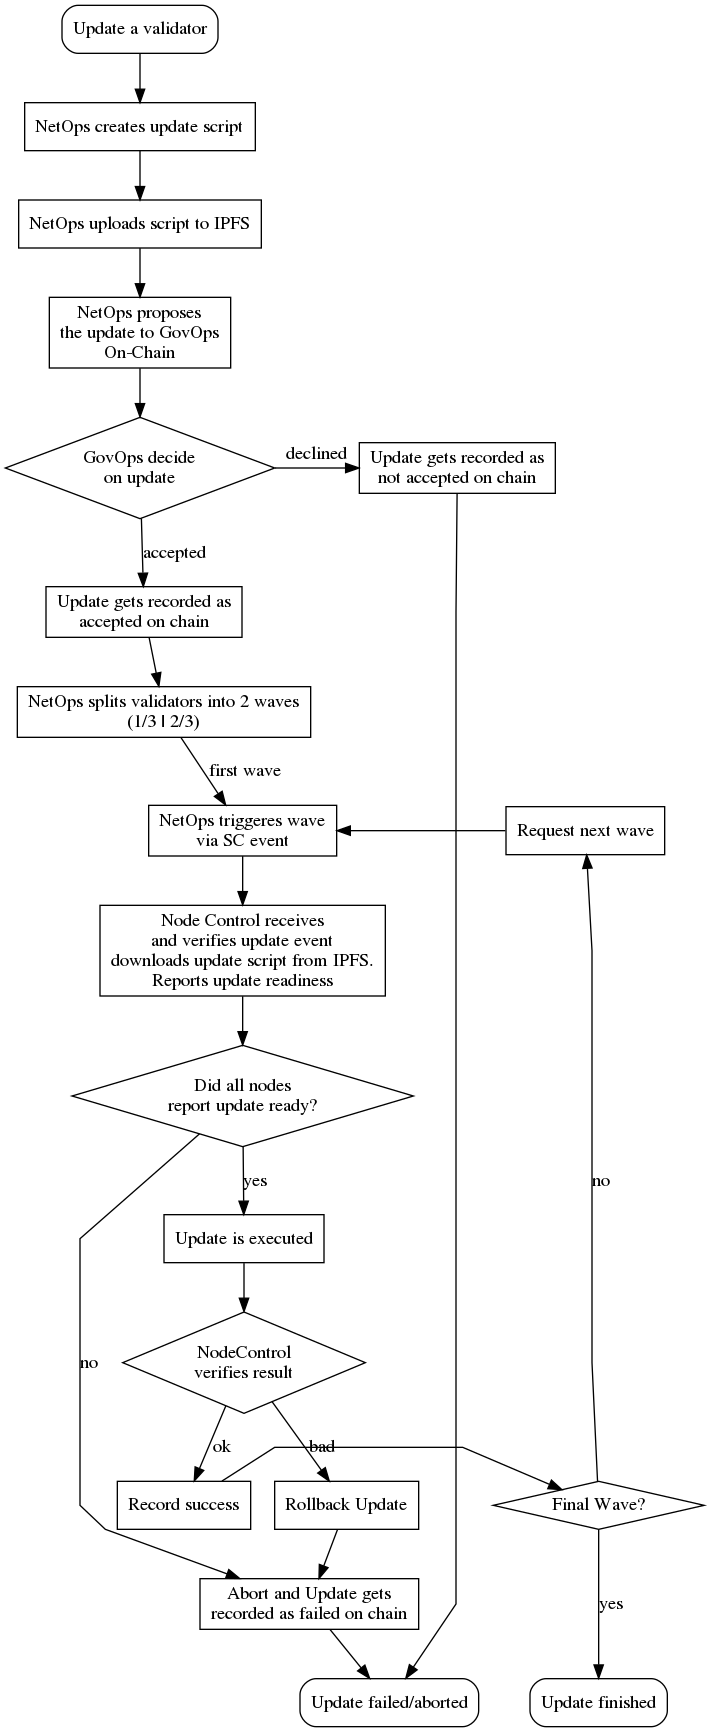
\includegraphics[width=\textwidth,height=\textheight,keepaspectratio]{./images/flow-update-validator.png}
	\caption{Update Flow}
	\label{fig:updateflow}
\end{figure}

Most updates will be executed automatically through NodeControl.

If the affiliate does not carry out the upgrade procedures during the time frame, NetOps will escalate the matter to GovOps which then will decide upon the removal of the authority node from the validator set.



\end{document}
